\documentclass[a4paper,12pt,ngerman]{scrartcl}
\usepackage{babel}
\usepackage{mathptmx}
\usepackage[T1]{fontenc}
\usepackage[utf8x]{inputenc}
\usepackage[a4paper,lmargin=2.5cm,rmargin=2.5cm,tmargin=2.0cm,bmargin=3.5cm,footskip=1.5cm]{geometry}
\usepackage{amsmath}
\usepackage{amssymb}
\usepackage{graphicx}
\usepackage{hyperref}

\hypersetup{
  colorlinks   = true, %Colours links instead of ugly boxes
  urlcolor     = blue, %Colour for external hyperlinks
  linkcolor    = blue, %Colour of internal links
  citecolor    = red %Colour of citations
}

\addtokomafont{sectionentry}{\normalfont}
\addtokomafont{section}{\normalfont}
\addtokomafont{subsection}{\normalfont}

\setcounter{tocdepth}{2}

\graphicspath{ {./images/} }

\renewcommand{\baselinestretch}{1.5} 

\begin{document}
\begin{titlepage}
	Projekttitel: Debuggen mit KI
	\vspace{1cm}
	
	Teilnehmende: PLACEHOLDER
	
	Erarbeitungsort: Zuhause
	
	Projektbetreuende: PLACEHOLDER
	
	Thema des Projekts: Kann eine KI beim Debuggen eines Programms helfen?
	
	Fachgebiet: Informatik
	
	Wettbewerbsparte: Jugend forscht
	
	Bundesland: PLACEHOLDER
	
	Wettbewerbsjahr: 2024
	
	\vspace{2cm}
	\vfill
\end{titlepage}
\clearpage
\tableofcontents
\clearpage

\section{Fachliche Kurzfassung}

Unsere Frage ist es, ob es möglich ist, dass eine KI für einen Programmierer den Debug Prozess übernimmt und selbstständig im Code den Grund für gegebene Fehler finden kann, ähnlich dazu, wie man es als Programmierer tun würde. Hierzu fügen wir eine Middleware in den Debug Prozess von VSCode zwischen Editor und Debug Adapter ein, welcher in der Kommunikation des Debuggers Nachrichten mitlesen, unterbrechen und hinzufügen kann. Eine große Herausforderung ist, wie die KI mit dieser Middleware kommunizieren wird, da LLMs nur Text Nachrichten empfangen und zurücksenden können. Wir benötigen also eine Konvertierung zwischen dem Debug Adapter Protokoll (DAP) und einem für die KI interpretierbaren und produzierbaren Text.

Um den Debug Prozess auf diese Art und Weise verändern zu können, entwickeln wir eine VSCode Extension, die beim Starten des Debug Adapters die Funktionen, die zur Kommunikation benutzt werden, mit eigenen Funktionen ersetzt, welche mit der KI kommunizieren und Nachrichten weiterhin mit den originalen Funktionen an den Editor oder an den Debug Adapter senden können.

Nun müssen die Daten des Debug Adapters (DA) in für die KI verständliche Begriffe übersetzt werden. Hierfür stellen wir der KI verschiedene Kommandos zum Empfangen oder Senden zur Verfügung, die von einem Übersetzer in DAP Nachrichten umgewandelt werden. Die KI kann so beispielsweise Breakpoints setzen, das Programm weiterlaufen lassen, oder den Wert einer Variable erfragen. Folgende Kommandos haben wir der KI zum Senden zur Verfügung gestellt:
\begin{itemize}
	\item ``BREAKPOINT [Zeile] [Datei]'' (setzen eines Breakpoints)
	\item ``CONTINUE'' (Programm weiterlaufen lassen)
	\item ``STEP'' (Einen Programmschritt ausführen)
	\item ``STEPINTO'' (In einen Funktionsaufruf eintreten)
	\item ``STEPOUT'' (Aus einem Funktionsaufruf austreten)
	\item ``VARIABLE [Name]'' (Variablen auslesen)
	\item ``LINE [Zeile] [Datei]'' (Einzelne Zeilen von Dateien auslesen)
	\item ``ERROR [Fehlermeldung]'' (Wenn die KI, nachdem sie die Anweisungen erhalten hat, irgendetwas vom debuggen abhält)
	\item ``CAUSE [Beschreibung]'' (Wenn schlussendlich der Grund für den Bug gefunden wurde).
\end{itemize}
Außerdem kann die KI folgendes Kommando erhalten:
\begin{itemize}
	\item ``PAUSED [Zeile] [Spalte] [Datei]'' (Wenn das Programm pausiert).
\end{itemize}

Zum Testen dieser KI haben wir sie mit verschiedenen Bugs ausprobiert und jeweils beurteilt, wie hilfreich die Antwort der KI zum Beheben der Bugs war. Hierbei sind wir zum Schluss gekommen, dass die KI mit den gegebenen Kommandos in der Lage ist, erfolgreich Breakpoints zu setzen und anschließend Schrittweise durch ein Program durchzugehen, wodurch es einfache Bugs finden und beschreiben kann. Allerdings ist uns auch aufgefallen, dass die KI mit den gegebenen Kommandos noch Probleme hat komplexere Datenstrukturen im Code nachzuvollziehen.

Aus unseren Ergebnissen schließen wir, dass KIs bereits heute in der Lage sind, den Debug Prozess zu übernehmen und zu steuern, allerdings scheinen sie mit unserer Implementation noch nicht in der Lage zu sein, komplexere Bugs zu finden. Aus diese Grund sehen wir aber in diesem Bereich auch noch viel Potenzial für weitere Entwicklung, um die KI besser als Debugger einsetzen zu können.

Der Code für unser Projekt ist öffentlich auf GitHub verfügbar: \url{https://github.com/Papierkorb2292/AI-Debugger}

\section{Motivation und Fragestellung}

Mit den letzten Fortschritten und dem öffentlichen Zugang zu KI, werden viele Möglichkeiten untersucht, wie eine KI Menschen helfen kann, und unter anderem beim Programmieren wurden bereits verschiedene hilfreiche Produkte entwickelt, die KI zum Unterstützen der Programmierenden verwenden. So gibt es beispielsweise schon länger die Möglichkeit Code Vorschläge von einer KI wie Tabnine oder Github Copilot zu erhalten und mit LLMs, wie ChatGPT, lässt sich auch ein ganzer Codeblock automatisch schreiben.

Wir haben uns gefragt, ob KI Programmierenden auch beim Debuggen von bereits geschriebenen Programmen helfen kann. Die KI ``Devin'' kann bereits selbst Programme schreiben und debuggen, benutzt allerdings zum debuggen \texttt{print} Statements, um den Zustand des Programms zu überwachen, indem dieser stellenweise in die Textausgabe geschrieben wird. Unser Ziel ist es jedoch die KI mit einem Debug Server, den auch Programmierende in ihrem Editor häufig benutzen, kommunizieren zu lassen. Ein weiterer Vorteil hiervon ist, dass es möglich wäre selbst zusammen mit der KI zu debuggen, indem man die KI nur Teile des Debuggen übernehmen lässt, und man den Rest noch selbst über den Editor vornimmt.

\section{Hintergrund und theoretische Grundlagen}

\subsection{KI}

Als KI (Künstliche Intelligenz) bezeichnet man häufig Verfahren zur Datenverarbeitung, für die keine genaue Handlungsanweisung festgelegt werden, sondern die mit Hilfe von Maschinellen Lernen erstellt wird, was einfach gesagt bedeutet, dass man die Parameter des Verfahrens stückweise ändert, um bei Eingangsdaten, für die schon Ausgangsdaten bekannt sind, die Ausgangsdaten des Verfahrens so nah wie möglich an die Erwarteten zu bekommen$^1$. Oft liegt der KI ein neuronales Netzwerk zugrunde, in welchem Eingangsdaten über mehrere Iterationen hinweg verschieden gewichtet und addiert werden können, um am Ende auf die Ausgangsdaten zu kommen.

Als LLM (Large Language Model) bezeichnet man KIs, die Textdaten verarbeiten und auf solche trainiert sind$^3$. Ein bekanntes Beispiel ist ChatGPT: Eine KI, welcher der Benutzer Textanfragen schreiben kann, und die dann selbst eine Textantwort produziert. LLMs zeichnen sich zudem durch ihre Flexibilität aus, da sie viele verschiedene Aufgaben über Text erledigen können und die Möglichkeit haben, viele Fragen zu beantworten$^2$.

\subsection{Debugging}

Beim Debuggen eines Programm mit einem Debugger, verbindet sich der Editor mit einem Debug Server, der das Programm ausführt und das Programm auch pausieren kann, damit der Editor den Zustand des Programms zu einem bestimmten Punkt anzeigen kann. Während das Programm pausiert ist, lässt sich außerdem mit dem Editor Schritt für Schritt durch das Programm durchgehen, um die Änderungen im Zustand des Programms zu beobachten.

Ein Debugger wird von Programmierenden benutzt, um Fehler in einem Program zu finden, indem man schrittweise durch das Programm durchgeht und dabei dessen Zustand überwacht, sodass man den Ort im Programm findet, bei dem der Zustand des Programms nicht mehr dem erwarteten Zustand entspricht. Mit Hilfe der dabei gewonnenen Informationen lässt sich gezielter nach dem Fehler suchen. 

\subsection{Debug Adapter}

Weil ein Debug Server direkt mit dem auszuführenden Programm interagiert, ist die Schnittstelle zum Debug Server oft spezifisch zur Sprache des Programms. Um den Editor mit dem Debug Server zu verbinden, wird deshalb ein Debug Server Adapter benutzt, der spezifisch zu einem Debug Server ist, und für welchen die Kommunikation mit dem Editor von Microsoft auf das Debug Adapter Protokoll (DAP) festgelegt wurde. Für jeden Debug Server kann so auch ein Debug Adapter angeboten werden, der mit dem Debug Server kommunizieren kann$^4$.

Folgendes ist eine Veranschaulichung, wie der Debug Prozess also aufgebaut ist:

\begin{center}
	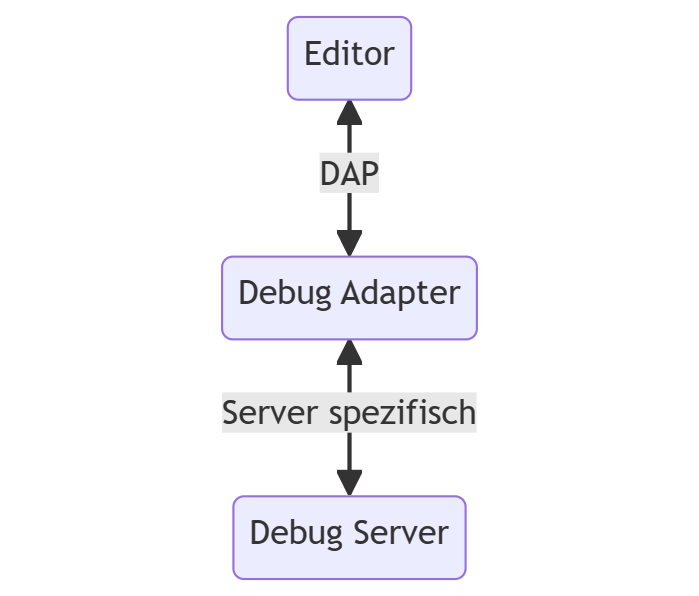
\includegraphics[width=0.5\textwidth]{debugger}
\end{center}

\section{Vorgehensweise, Materialien und Methoden}

Um zu testen, ob es möglich ist, eine KI auf diese Art und Weise beim Debuggen unterstützen zu lassen, werden wir selbst unsere Idee als VSCode Extension umsetzen, und verschiedene Ansätze, um mit der KI zu interagieren, ausprobieren.

Um eine KI in den Debug Prozess zu interagieren, fügen wir zunächst eine Middleware zwischen Editor und Debug Adapter hinzu, durch welche alle Nachrichten zwischen dem Editor und Debug Adapter laufen, damit die KI diese beobachten und unterbrechen kann. Außerdem wird es hiermit möglich, Nachrichten, die durch die KI eingebracht werden, an den Editor und Debug Adapter zu senden. Dies macht es möglich für die KI, Kontrolle über den Debug Prozess zu nehmen.

Es gibt verschiedene Möglichkeiten, wie die KI selbst laufen kann. Zunächst werden wir von OpenAI das KI Modell GPT-4o benutzen, mit welchem man über das Internet kommuniziert. Es wäre außerdem möglich später verschiedene KI Modelle auszuprobieren, um zu testen, wie gut verschiedene Modelle debuggen können.

\subsection{KI Debugger Dienst}

Der wichtigste Teil ist allerdings, wie die KI mit ihren Nachrichten mit dem Benutzer, dem Editor und dem Debug Adapter kommuniziert. Der Benutzer muss nämlich die Möglichkeiten haben, Nachrichten an die KI zu senden, die KI muss antworten können, und zusätzlich muss eine Übersetzung zwischen DAP Nachrichten (normalerweise werden diese zwischen Editor und Debug Adapter gesendet) und dem Text, über welchen die KI kommuniziert, stattfinden. Im folgenden wird dieser Teil als ``KI Debugger Dienst'' betitelt. Außerdem muss der Editor den Kontext, also beispielsweise den Inhalt der Dateien, in denen gedebuggt wird, an den KI Debugger Dienst senden, damit dieser weiß, welche Positionen in den Dateien den verschiedenen Teilen des laufenden Programms entsprechen, um an diesen Stellen pausieren zu können und den Kontext einer Pause zu verstehen.

Folgendes Diagramm veranschaulicht den nun erweiterten Aufbau des Debuggers zusammen mit der Kommunikation mit der KI.

\begin{center}	
	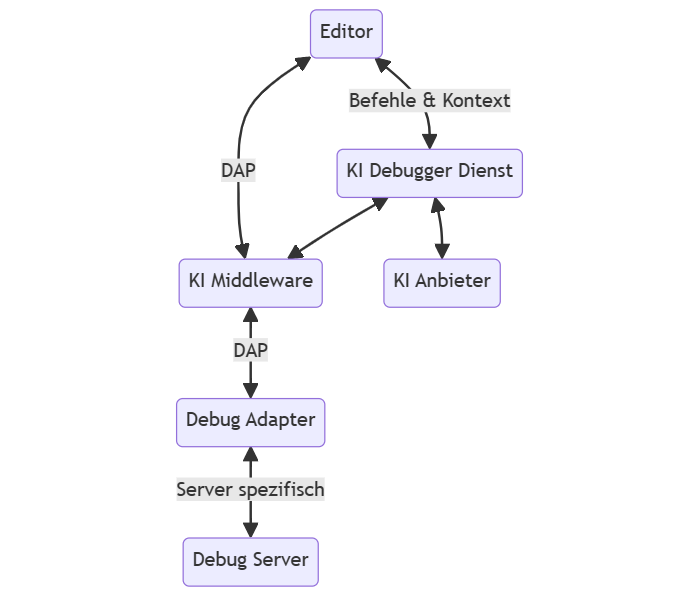
\includegraphics[width=0.875\textwidth]{ai_integration}
\end{center}

Um zu verstehen, wie die Kommunikation zwischen dem Debug Adapter und dem KI-Debugger-Dienst funktioniert, betrachten wir erstmal genauer, wie der KI-Debugger-Dienst die verschiedenen Nachrichten verarbeitet:

Da DAP Nachrichten im JSON Format gesendet werden und dabei oft viele Informationen über den Zustand des Programms enthalten, bei denen wichtig ist, dass sie akkurat sind, wie Dateipfade, Breakpoint Ids, etc., haben wir uns dagegen entschieden, die KI direkt diese JSON Objekte lesen und auslesen zu lassen, da dann die KI viel mehr Wert darauf legen müsste, vollständig fehlerfreie JSON Objekte auszugeben, was die Qualität des eigentlichen Debuggens beinträchtigen könnte.

Stattdessen haben wir uns überlegt, die KI mit dem KI Debugger Dienst über simple Textnachrichten kommunizieren zu lassen, von denen jede ein Kommando darstellt. So ein Kommando ist aufgebaut aus einem Kommando Namen und einer Liste von Argumenten, die das Kommando benötigt. Beispielsweise haben wir das Kommando ``BREAKPOINT [Zeile] [Datei]'' erstellt, welches der KI erlaubt einen Breakpoint in einer bestimmten Datei und Zeile zu setzen, was bedeutet, dass das Programm pausiert, wenn es diese Zeile erreicht. Über die gleiche Art und Weise werden auch bestimmte Events der KI mitgeteilt, indem die KI beispielsweise das Kommando ``PAUSED [Zeile] [Spalte] [Datei]'' erhält, sobald das Programm pausiert.

Alle der KI zur Verfügung stehenden Kommandos werden ihr in der ersten Nachricht mitgeteilt, zusammen mit ihrem Sinn als Debugger und dem zu behebenden Bug. Das Vermitteln der Kommandos geschieht hierbei durch festgelegte Sätze, diese Kommandos werden also in eine sprachliche Form gebracht, die die Kommunikation mit dem LLM ermöglicht. Beispielsweise entspricht das Kommando ``BREAKPOINT'' dem Satz: ``You can set breakpoints in the code by starting your message with "BREAKPOINT" followed by the line number and the file name.'' Dieses Prinzip wird auf jedes Kommando angewendet. Nun, da die Befehle für die KI vorliegen, werden diese übermittelt und die Antworten empfangen. Die jeweiligen Antworten sind so formatiert, dass sie ohne großen Aufwand weiterverarbeitet werden können.

Da wir davon ausgehen, dass die KI nicht immer die Fragestellung ausreichend verstehen wird (unter anderem, wenn der zu findende Bug nicht gut genug beschrieben wird), haben wir ihr außerdem die Möglichkeit gegeben, Fehler auszugeben, indem sie das Kommando ``ERROR [Fehlermeldung]'' sendet. Dieses Kommando wird an den Editor weitergeleitet, sodass ein User die Fehlermeldung sehen kann und die Anfrage anpassen kann.

Wie bereits erwähnt ist es außerdem wichtig, dass die KI Zugriff auf den Code des Programs bekommt. Auch hierfür gibt es ein Kommando, welches eine Zeile aus einer Datei zu der KI senden kann, wenn die KI ``LINE [Zeile] [Datei]'' sendet. Hierbei meiden wir, eine gesamte Datei auf einmal an die KI zu senden, da dies darfür sorgen könnte, dass die KI sich nicht den genauen Inhalt der einzelnen Zeilen richtig merken kann. Außerdem würde, wenn man der KI eine ganze Datei senden würde, dies viele Tokens verbrauchen, was schlussendlich dafür sorgen würde, dass der Debug Prozess mehr Geld köste (Siehe \autoref{sec:compression} \nameref{sec:compression}).

\subsection{Einbinden der KI}

Dieses Kommando System muss nun in den Debug Prozess eingebunden werden, da im Moment noch das Erhalten und Senden von Kommandos unabhängig vom Debuggen passiert. Hierfür haben wir der KI zusätzlich folgende Kommandos zur Verfügung gestellt, mit Hilfe derer sie ähnlich wie der User mit dem Debug Prozess interagieren kann: ``CONTINUE'', ``STEP'', ``STEPINTO'', ``STEPOUT''. Jeder dieser Kommandos entspricht einem Knopf im Editor, den der Benutzer drücken kann, um das Programm weiterlaufen zu lassen, oder um Schritt für Schritt durch das Programm zu gehen. Wenn die KI ein solches Kommando sendet, wird eine entsprechende DAP Nachricht an den Debug Adapter gesendet, während außerdem eine Nachricht an den Editor gesendet wird, die diesem sagt, der Debug Adapter wäre von alleine weitergelaufen, sodass der User den Verlauf des Debuggens gut mitverfolgen kann.

Während in Folge eines dieser Kommandos das Program weiterläuft, bis es am nächsten Breakpoint angekommen ist oder den angeforderten Schritt ausgeführt hat, wird hingegen die Konversation mit der KI pausiert. Diese geht erst weiter, wenn das Programm wieder pausiert hat, woraufhin die bereits genannte ``PAUSED'' Nachricht an die KI gesendet wird. Auf diese Art und Weise erhalten wir eine Art Rückkopplung, die abwechselnd den Debug Prozess oder die KI laufen lässt und so der KI das schritthafte Debuggen ermöglicht.

Ein zusätzliches wichtiges Kommando ist ``VARIABLE [Name]'', welches der KI erlaubt den Wert einer Variable zu erfragen, sodass die KI den Zustand des Programms aktiv verfolgen kann und dadurch direkt Rückschlüsse darauf ziehen kann, an welcher Stelle im Code der Zustand vom erwarteten Zustand abweicht.

Zuletzt hat die KI außerdem ein ``CAUSE [Beschreibung]'' Kommando, mit dem sie zum Abschluss den von ihr herausgefunden Grund ausgeben kann, warum der Bug aufgetreten ist.

\subsection{Komprimierung der Konversation}
\label{sec:compression}

Ein weiterer wichtiger Aspekt ist die Komprimierung der übermittelten Daten. Dies ist aufgrund des Bezahlmodells von OpenAI wichtig, das nach dem Prinzip sogenannter 'Tokens' fungiert, für deren Anzahl man bezahlt$^7$. Dieser Prozess heißt Tokenisierung und funktioniert nach Folgender Reihenfolge:
\begin{enumerate}
	\item Normalisierung des Textes: Im Kern wird hier nichts weiter gemacht als Großbuchstaben in Kleinbuchstaben umgewandelt und unnötige Leerzeichen entfernt werden.
	\item Aufteilung: Der normalisierte Text wird nun in Wörter zerlegt. Dies kann durch das Aufteilen an Leerzeichen und Satzzeichen geschehen.
	\item Tokenisierung: Der nun vorliegende Text wird zum Schluss von Algorithmen zerlegt und in Tokens mit einer vordefinierten ID eingeteilt. Aufgrund dieser ID ist es dem GPT Modell möglich das Wort zu interpretieren.
\end{enumerate}

Beispielsweise wird der Satz ``Die Abkürzung für Künstliche Intelligenz ist KI'' in folgende 16 Tokens aufgeteilt$^{10}$:\\
\texttt{Die| Ab|k|ür|zung| für| K|ünst|liche| Int|ell|igen|z| ist| K|I}

Unser Ziel ist also so viel sogenannte 'one-word-tokens' zu verwenden wie möglich. Um das zu erreichen, benutzen wir KI, speziell das ChatGPT-4o Modell, um Prompts zu optimieren.

\subsection{Erheben von Daten}

Da nun die KI in den Debug Prozess integriert wurde, ist der nächste Schritt die Erfolgsrate der KI beim Debuggen herauszufinden. Hierfür benötigen wir Beispielprobleme, mit denen wir die KI testen können. Außerdem haben wir vor, die Schwierigkeit eines Problems bewerten zu können, sodass wir die Erolgsrate der KI in Abhängigkeit der Schwierigkeit des Problems erheben können. Hierzu haben wir uns überlegt, verschiedene Aufgaben von Advent of Code zu lösen und mit der KI Bugs in unseren Lösungen zu debuggen. Advent of Code ist ein jährlicher online Adventskalender mit 25 Programmieraufgaben, die von Tag zu Tag schwieriger werden$^{11}$. Jeder Tag besteht dabei aus zwei Aufgabenteilen. Wir haben uns dazu entschiedenen aus dem Kalender von 2023, alle geradzahligen Tage bis einschließlich Tag 12 zu lösen. Wir beschränken uns auf die geradzahligen Tage, da es keinen großen Unterschied zwischen den einzelnen Tagen geben sollte und wir somit einen größeren Schwierigkeitsbereich in der gleichen Zeit untersuchen können. Außerdem haben wir 2023 gewählt, da dies noch nach dem Cutoff Datum für die von uns verwendete KI ist (ChatGPT-4o), was bedeutet, dass keine Lösungen für die Aufgaben in ihren Trainingsdaten enthalten sind. Dies sollte die Ergebnisse realistischer machen, da beim Verwenden der KI für echte Bugs ebenfalls mindestens relevante Teile des Programs nicht in den Trainingsdaten enthalten sind. Wir vermuten, dass die KI besser in der Lage ist, Bugs in den Aufgaben vom Anfang des Dezembers als später im Dezember zu finden, da die Aufgaben später im Dezember meist komplexer sind.

Außerdem vermuten wir, dass es einfacher ist für die KI Tippfehler zu finden, anstatt Logikfehler zu finden, da sich Tippfehler meist bereits aus dem Code rauslesen lassen, wohingegen für Logikfehler meist der genaue Zustand des Programs an der richtigen Stelle überwacht werden muss. Tippfehler heißt hierbei, wenn nur ein paar Zeichen im Code falsch eingegeben wurden, wohingegen Logikfehler bedeutet, dass der Lösungsansatz falsch ist oder bestimmte (Sonder-)Fälle nicht behandelt. Um diese Vermutung zu überprüfen, testen wir die KI in jedem Aufgabenteil der 6 Tage einmal mit einem Tippfehler und einmal mit einem Logikfehler.

Die Bugs mit denen wir die KI testen sind entweder uns selbst beim Lösen der Aufgaben passiert, oder wir haben sie absichtlich in den Code eingebaut, falls uns kein Fehler beim Lösen der Aufgabe unterlaufen ist. Des weieteren werden wir beurteilen, wie verständlich und hilfreich die KI den Grund für den Bug formulieren kann.

\section{Ergebnisse}

Alle Test Funktionen und die Ergebnisse der KI sind unter folgendem Link zu finden TODO: \url{https://github.com/Papierkorb2292/AI-Debugger/blob/c08f8f01a267f1b80094e715a3c8b819b1061ae7/testWorkspace/test.py}

Folgende Tabelle zeigt für jeden der getesteten Tagen, ob die jeweilige Art von Bug in den Aufgabenteilen erfolreich durch die KI bestimmt werden konnte. Hierbei haben die Zeichen in der Tabelle folgende Bedeutung:
\begin{enumerate}
\item X_V (Vollständig): Der Ort des Bug und eine vollständige bzw. zum Lösen hinreichende Beschreibung der Ursache war in der Antwort der KI enthalten
\item X_O (Ort): Nur der Ort des Bugs, aber keine hilfreiche Beschreibung war in der Antwort der KI enthalten.
\item X_E (Extra Info): Eine hilfreiche Beschreibung des Bugs war in der Antwort der KI enthalten, allerdins erst, nachdem der initialien Prompt ein extra Verweis auf bestimmte Programmstellen hinzugefügt wurde, in denen der Bug zu finden ist.
\item _T (Tokens): Der Bug ließ sich nicht mit der KI bestimmen, weil der Debug Prozess zu viele Schritte benötigte, was die KI Konversation sehr lang und damit teurer gemacht hat, weshalb wir den Debug Prozess unterbrochen haben. Dies ist oft bei Schleifen passiert, die hätten übersprungen werden können. Stattdessen war die Antwort der KI, die Schleife schrittweise zu durchgehen, ohne das 'EVAL' Kommando für das Vearbeiten von Variablenwerten zu verwenden.
\item _B (Beendet):   Der Bug ließ sich nicht mit der KI bestimmen, weil die KI das Program verlassen hat ohne den Bug zu beschreiben
\item _F (Fehlerhaft): Der Bug ließ sich nicht mit der KI bestimmen, weil die Antwort den KI den Bug fehlerhaft beschrieben hat oder einen gar nicht vorhandenen Bug beschrieben hat.
\end{enumerate}
\begin{center}
\begin{tabular}{|c|c|c|c|c|c|c|}
	\hline
 	Tag                 &  2  &  4  &  6  &  8  & 10  & 12  \\
	\hline
	Teil 1, Logikfehler & X_V & X_O &  _F & X_O &  _B &  _T \\
	Teil 2, Logikfehler & X_V & X_V & X_E & X_V &  _T &  _F \\
	Teil 1, Tippfehler  & X_V & X_V &  _F &  _F &  _F &  _T \\
	Teil 2, Tippfehler  & X_V &  _F & X_O & X_V &  _T & X_V \\
	\hline
\end{tabular}
\end{center}

Insgesamt konnten mit dem KI Debugger über 12 Teilaufgaben also 7 Logikfehler und 6 Tippfehler gefunden werden.

Folgende zwei Situationen waren für uns besonders interessant:
\begin{enumerate}
\item Tag 8 - Teil 2 - Logikfehler: Hier war die Lösung der Aufgabe das Berechnen des kleinsten gemeinsamem Vielfachen von einer Liste an Zahlen. Der Bug, mit dem die KI getestet wurde, ist, dass stattdessen alle Zahlen der Liste zusammenmultipliziert wurden. Die Antwort der KI enthielt hierbei direkt, dass stattdessen das KGV berechnet werden muss, ohne, dass ein Verweis auf das KGV in der initialen Prompt enthalten war. Die KI hat demnach ohne besondere Information die Beschreibung der Aufgabe mit dem KGV in Verbindung gebracht.
\item Tag 10 - Teil 2: Diese Bugs konnten nicht mit der KI gelöst werden. Die Lösung der Aufgabe bestand aus mehreren Schleifen, die nacheinander ausgeführt werden. Dies stellt ein Problem für unseren KI Debugger dar, weil die KI oft nur viele einzelne ``STEP'' Kommandos ausgibt, um eine Schleife zu überspringen, anstatt einen Breakpoint nach dem Ende der Schleife zu setzen. Dies führt zu längeren Konversationen und Debug Prozessen, die somit mehr Geld und Zeit kosten. Außerdem haben wir bei mehreren Versuchen beobachtet, dass, wenn die Schleife zurück an den Anfang gesprungen ist, sich die Zeilennummern in von der KI ausgegebenen ``LINE'' Kommandos weiterhin erhöht haben. Die Antworten der KI schienen dann Kommandos basierend auf der zuletzt eingelesen Zeile auszugeben, anstatt für die Zeile, bei der sich das Program gerade befindet (die Benachrichtigung für jedes Pausieren des Debuggers enthält aber diese Zeilennummer). Beispielsweise hat die KI ``STEPINTO'' Kommandos ausgegeben, wenn eine Zeile mit einem Funktionsaufruf eingelesen wurde, obwohl die Zeile, wo das Program eigentlich pausiert war, keinen Funktionsaufruf enthielt.
\end{enumerate}

\section{Ergebnissdiskussion}

Die Ergebnisse sind vielversprechend, da sie zeigen, dass es heutigen KIs bereits möglich ist die grundlegende Funktionsweise von Debug Prozessen zu reproduzieren. Außerdem hat sich unsere Vermutungen bewahrheitet, dass sich Bugs in einfachen Aufgaben (von den ersten paar Tagen in Advent of Code 2023) besser mit der KI finden lassen, als Bugs in schwereren Aufgaben (von den späteren Tagen in Advent of Code 2023).

Allerdings lässt sich mit den von uns erhobenen Daten nicht klar bestätigen, dass sich von uns als Tippfehler eingeordete Bugs einfacher mit der KI finden lassen, als von uns als Logikfehler eingeordnete Bugs, da aus den erhobenen Daten kein klarer Unterschied in der Erfolgsrate von Tippfehlern und Logikfehlern hervorgeht. Daraus schließen wir, dass die Art von Bug nicht das hauptsächliche Problem für unseren KI Debugger darstellt, sondern die Komplexität des Programms und die Art, wie der KI Debugger durch das Programm navigieren kann, um die fehlerhafte Stelle zu finden. Beispielsweise fanden wir durch unsere Tests heraus, dass die Verwendung von mehreren Schleifen die KI daran hindern kann, den Grund des Bugs zu finden, weil die KI nicht gut in der Lage zu sein scheint, die Position, bei der sich das Program gerade befindet, zu verfolgen, sondern stattdessen Antworten basierend auf der zuletzt eingelesenen Zeile erstellt. Wir vermuten, dass der Grund, warum die KI auch bei einem Zurückspringen der Schleife weiterhin nachfolgende Zeilen einliest, darin liegt, dass die KI nur das Muster der vorherigen ``LINE'' Kommandos, bei denen sich die Zeilennummer immer um 1 erhöht, fortsetzt.

Eine mögliche Verbesserung, die wir uns zum besseren Einlesen des Programs und Navigieren über Schleifen hinweg überlegt haben, ist dass die KI nicht direkt mit dem Debuggen anfängt, sondern zunächst selbstständig relevante Sektionen des Programs einliest, um Stellen im Code auszugeben, die genauer auf den Bug untersucht werden sollten. Dies ähnelt auch mehr dem normalen Debug Vorgang durch Programmierende, welche zuerst den Code durchgehen, um Stellen zu finden, wo sie einen Bug vermuten würden. Anschließend könnte die KI wieder Kommandos ausgeben, um das Program (vielleicht merhmals) zu starten und zu warten, bis es bei der relevanten Stelle pausiert, sodass dann wieder wie zuvor mit dem Debugger durch das Program durchgegangen und der Zustand des Programs überwacht werden kann.

\section{Fazit und Ausblick}

\subsection{Fazit}

Zusammengefasst lässt sich sagen, dass wir mit unserem System erfolgreich eine KI in den Debug Prozess zu integrieren konnten, und, dass diese KI in der Lage ist, den Debug Prozess zu kontrollieren. In einer solchen Integration sehen wir viele Entwicklungsmöglichkeitein, um einen KI Debugger als ein für Programmierende nützliches Tool bereitzustellen. Wir sind zum Schluss gekommen, dass, auch wenn im Verlaufe der Tests noch weitere Herausforderungen offentsichtlich geworden sind, die KI mit verbesserten Prompts und mehr Kommandos für noch mehr Kontrolle über den Debug Prozess auch kompliziertere Bugs finden könnte, da es bereits andere KIs, wie Github Copilot gibt, die Code einlesen und benutzbaren Code ausgeben können (womit sie bereits für Programmierende ein nützliches Tool sind), was zeigt, dass es manchen heutigen KIs bereits möglich ist eine Beschreibung einer Aufgabe mit dem zur Umsetzung notwendigem Code zu verbinden. Würde eine KI, die in einem solchen Ausmaß auf Code trainiert worden ist, dass es die vielen einzelnen Bestandteile einer Codebase (also einem gesamten Projekt) ebenso mit der gestellten Aufgabe verknüpfen kann, ebenfalls die Möglichkeit gegeben werden, einen Debug Prozess zu steuern, erwarten wir eine beträchtliche Verbesserung in der Leistung des KI Debuggers.

\subsection{Ausblick}

Zunächst möchten wir darauf aufmerksam machen, dass mehr und realistischere Tests zur genaueren Evaluierung der Nützlichkeit des KI Debuggers notwendig sind, da wir sie nur auf eine kleine Anzahl an Bugs getestet haben, welche außerdem nicht von richtigen Projekten stammen. Hierfür wäre es entweder möglich bei einer Gruppe von Programmierenden über einen längeren Zeitraum Bugs zu sammeln, auf welche dann die Debugger KI getestet werden kann, oder über öffentliche Code Repositories, wie Github, Bugs zu sammeln, da es dort meist eine Liste von gefundenen Fehlern gibt, mit denen die KI getestet werden könnte.

Wir erwarten außerdem, dass sich wesentlich bessere Ergebnisse erzielen lassen würden, wenn man anstatt einer allgemeinen KI, die auf viele verschiedene Aufgaben trainiert ist, eine KI spezifisch für das Debuggen trainiert. Es wäre beispielsweise möglich, diese KI auch auf die Syntax von Programmiersprachen spezialisiert zu trainieren, sodass sie das Program und die Aufgabe besser versteht. Ein möglicher Start hierfür wäre die KI ``Codex'' von OpenAI, die speziell auf das Verständis von Code trainiert ist. Dies ist auch das KI Modell, auf welchem Github Copilot aufbaut.

Um zusätzliche Trainingsdaten für eine solche KI zu erheben, wäre es möglich, die Middleware bei normalen Debug Prozessen mitlaufen zu lassen, sodass die Kommunikation zwischen Editor und Debug Adapter aufgezeichnet wird. Das würde es erlauben die KI auf die aufgezeichneten Daten zu trainieren, sodass die KI schließlich den Editor und damit auch die Programmierenden nachstellt. Fraglich ist, ob es möglich wäre von den aufgezeichneten Daten auf das Problem und die Problemlösung zu schließen, oder ob es notwendig wäre, dass die Programmierenden, wenn sie ihre Debug Prozesse aufzeichnen möchten, auch zusätzliche Informationen über das Problem und die anschließend angewandte Lösung angeben müssten, sodass die KI dafür trainiert werden kann, das Problem einzulesen und die Lösung auszugeben.

Eine weitere große Verbesserungsmöglichkeit ist es, dem bereits von uns erstelltem System mehr Kommandos hinzuzufügen. Beispielweise könnte man es der KI möglich machen, eine Liste aller Variablen zu erhalten, den Call stack auszulesen (also die Reihenfolge der Funktionsaufrufe zu erhalten), den Wert einer Variable zu ändern, oder auch die Möglichkeit geben, das Programm neu zu starten, um Daten aus dem vorherigen Durchlauf in einem neuen Versuch, das Program zu debuggen, anwenden zu können. Dies sind Aktionen, die auch beim normalen Debuggen oft nützlich sind, und die es der KI ermöglichen könnten, das Programm besser zu debuggen.

\section{Quellen- und Literaturverzeichnis}

$^1$ Wikimedia Foundation Inc.,  ``Künstliche Intelligenz - Wikipedia'', grundlegende Information zu künstlicher Intelligenz\\
\url{https://de.wikipedia.org/wiki/K\%C3\%BCnstliche_Intelligenz}, besucht am 19.03.2024\\
$^2$ Wikimedia Foundation Inc.,  ``Large language model - Wikipedia'', grundlegende Information zu Large Language Models\\
\url{https://en.wikipedia.org/wiki/Large_language_model}, besucht am 19.03.2024\\
$^3$ Wikimedia Foundation Inc.,  ``Language model - Wikipedia'', grundlegende Information zu Language Models \\
\url{https://en.wikipedia.org/wiki/Language_model}, besucht am 19.03.2024\\
$^4$ Microsoft, ``Overview [über das Debug Adapter Protokol]'', grundlegende Information zum Debug Adapter Protokoll
\url{https://microsoft.github.io/debug-adapter-protocol/overview.html}, besucht am 25.03.2024\\
\vspace{1em}\\
$^5$ Microsoft, ``Extension API | Visual Studio Code Extension API'', Anleitung zum Entwickeln einer VSCode Extension\\
\url{https://code.visualstudio.com/api}, besucht am 19.03.2024\\
$^6$ Microsoft, ``vscode/blob/main/src/vs/workbench/contrib/debug/node/debugAdapter.ts at main microsoft/vscode'', VSCode Quellcode zur Kommunikation mit Debug Adaptern\\
\url{https://github.com/microsoft/vscode/blob/main/src/vs/workbench/contrib/debug/node/debugAdapter.ts}, besucht am 19.03.2024\\
$^7$ OpenAi, ``Introduction - OpenAI API'', Grundlegene Information zum Benutzen der KIs von OpenAPI\\
\url {https://platform.openai.com/docs/introduction}, besucht am 01.07.2024\\
$^8$ OpenAi, ``OpenAI Platform'', Information über\\
\url {https://platform.openai.com/organization/api-keys}, besucht am 01.07.2024\\
$^9$ OpenAi, ``ChatGPT'', Die ChatGPT KI\\
\url {https://chatgpt.com}, besucht am 01.07.2024\\
$^{10}$ OpenAi, ``Introduction - OpenAI API'', Tool zum Ausprobieren, in was für Tokens ein Text von OpenAI aufgeteilt wird\\
\url {https://platform.openai.com/tokenizer}, besucht am 01.07.2024\\
$^{11}$ Advent of Code, ``About - Advent of Code 2024'', Beschreibung der Advent of Code Webseite\\
\url {https://adventofcode.com/2024/about}, besucht am 23.01.2025\\
\end{document}